\section{Discover and visualize the system to gain insights}
\label{sec:ch2:discover}

So, now we've got a codebase accumulated to read in the input data, get it cleaned up, embed it while borrowing strength from all networks, and make some predictions. 

So, now we're finished, right?

Wrong! The end of a computational analysis typically means the fun is just beginning: it's now time to \emph{make sense} of whatever, exactly, it is that you just did!

How could we visualize the node clusters (or, more formally, called \emph{communities}) that we just made? We already known about the pairs plot, which we saw in Figure \ref{fig:ch2:mase}(B). 

What if we take a look at the nodes, which if we remember were areas of the brain, and visualize how they \emph{really} look in the brain's natural space?

It turns out that the areas of the brain corresponding to the nodes in your network are, in fact, \emph{known} 3D points in the brain. This means that, with some minor work, we can figure out the coordinates of the individual nodes for the brain. Let's use the neuroparc repository from \cite{Lawrence2021Mar} to grab the 3D coordinates of each node in the network. You don't need to worry too much about how this code works; at a high-level, it just obtains 3D coordinates for the nodes of the network in a \texttt{json} file, and then parses them into a \texttt{pandas} dataframe:


\begin{lstlisting}[style=python]
from urllib import request
import json
import pandas as pd

coord_dest = os.path.join(FMRI_PATH, "coordinates.json")
request.urlretrieve("https://github.com/neurodata/neuroparc/" + "raw/master/atlases/label/Human/Metadata-json/" + parcellation + "_space-MNI152NLin6_res-2x2x2.json", coord_dest);

with open(coord_dest) as coord_f:
    coords = []
    for roiname, contents in json.load(coord_f)["rois"].items():
        try:
            if roiname != "0":
                coord_roi = {"x" : contents["center"][0], "y" : contents["center"][1], "z" : contents["center"][2]}
                coords.append(coord_roi)
        except:
            continue
            
coords_df = pd.DataFrame(coords)
\end{lstlisting}

Now that we have the coordinates, let's try plotting the nodes, but in their native spatial orientation. Here, the color will indicate the predicted label, from our clustering. The slices we'll show will be a saggital slice through the brain. A saggital slice shows the brain nodes oriented from back (right of the plot) of the brain to front (left of the plot), and from bottom (bottom of the plot) to top (top of the plot). On the left, we show the brain with the lobe annotations, and on the right, the predicted labels of each node in color, where each node is shown in its true physical location:

\begin{lstlisting}[style=python]
import matplotlib.image as mpimg

coords_df["Community"] = labels
coords_df['Community'] = coords_df['Community'].astype('category')
fig, axs = plt.subplots(1, 2, figsize=(18, 6))
axs[0].imshow(mpimg.imread('./Images/lobes.png'))
axs[0].set_axis_off()
sns.scatterplot(x="y", y="z", data=coords_df, hue="Community", ax=axs[1])
\end{lstlisting}
\begin{figure}[h]
    \centering
    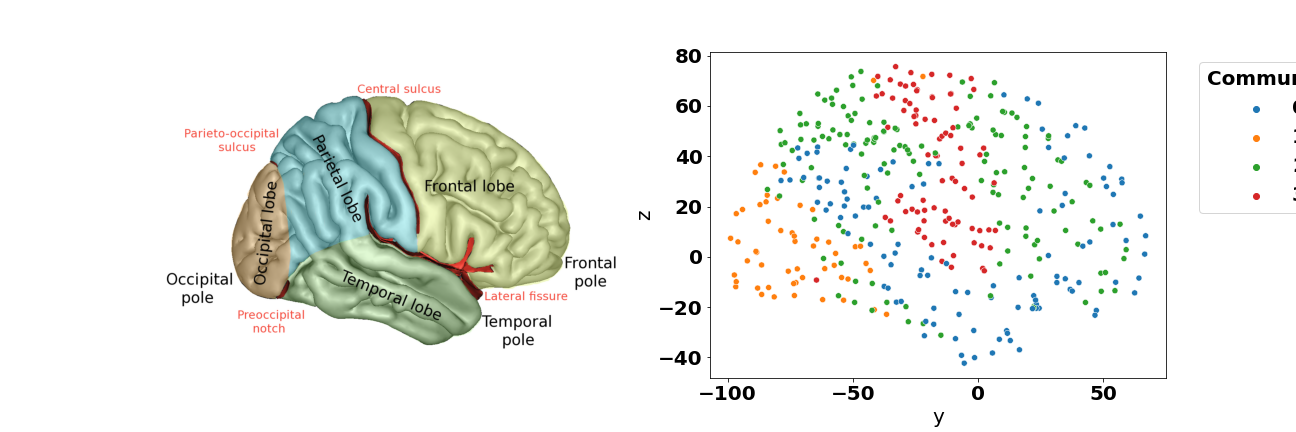
\includegraphics[width=\linewidth]{foundations/ch2/Images/brain_preds.png}
    \caption[Visualizing estimated node communities in 3D space]{Visualizing the estimated node communities with brain lobe annotations.}
    \label{fig:ch2:brain_preds}
\end{figure}

The resulting plot is shown in Figure \ref{fig:ch2:brain_preds}. So, the estimated communities of each node don't quite perfectly align with the brain lobe that the node is in. However, nodes in the tend to be \emph{spatially close} to other nodes in the same estimated community. Notice, for instance, that a lot of nodes in the left side of the brain, the part marked ``occipital lobe'' in the plot, tend to be the same color. In our plot, these nodes are orange; in your plot, they might be a different color. 

In neuroimaging, there tend to be ``groups'' of brain areas that work together, which are organized in files called ``parcellations''. The idea is that they ``parcellate'' (segment) different areas of the brain baesd on two factors: whether the areas of the brain work together, and whether they are located near each other in the brain. Let's see how well the labels we obtained align with these parcellations. We'll do this by looking at the different parcellations (there are $7$ of them in the one that we will use here), and count the number of nodes in a given community (the thing that you just estimated, indicated by color, above) that are assigned to a particular parcel as well. This means that we will end up with a matrix where the number of rows are the number of true parcels in the brain, the number of columns is the number of predicted communities that you found above, and the entries of the matrix are the counts of nodes in the network that are assigned to a given community \emph{and} fall into a given parcel:

\begin{lstlisting}[style=python]
import contextlib
import datasets.dice as dice
from sklearn.metrics import confusion_matrix
from graphbook_code import cmaps

group_dest = os.path.join("./datasets/", "Yeo-7_space-MNI152NLin6_res-2x2x2.nii.gz")
request.urlretrieve("https://github.com/neurodata/neuroparc/" + "blob/master/atlases/label/Human/" +
"Yeo-7_space-MNI152NLin6_res-2x2x2.nii.gz?raw=true", group_dest);
roi_dest = os.path.join("./datasets/", "Schaefer200_space-MNI152NLin6_res-2x2x2.nii.gz")
request.urlretrieve("https://github.com/neurodata/neuroparc/" + "blob/master/atlases/label/Human/" + "Schaefer400_space-MNI152NLin6_res-2x2x2.nii.gz?raw=true", roi_dest);

dicemap, _, _ = dice.dice_roi("./datasets/", "./datasets", "Yeo-7_space-MNI152NLin6_res-2x2x2.nii.gz", 
              "Schaefer200_space-MNI152NLin6_res-2x2x2.nii.gz", verbose=False, plot=False)
actual_cluster = np.argmax(dicemap, axis=0)[1:] - 1

# make confusion matrix
cf_matrix = confusion_matrix(actual_cluster, labels)

# and plot it
ax = sns.heatmap(cf_matrix, cmap=cmaps["sequential"])
ax.set_title("Confusion matrix")
ax.set_ylabel("True Label")
ax.set_xlabel("Predicted Label")
\end{lstlisting}

\begin{figure}[h]
    \centering
    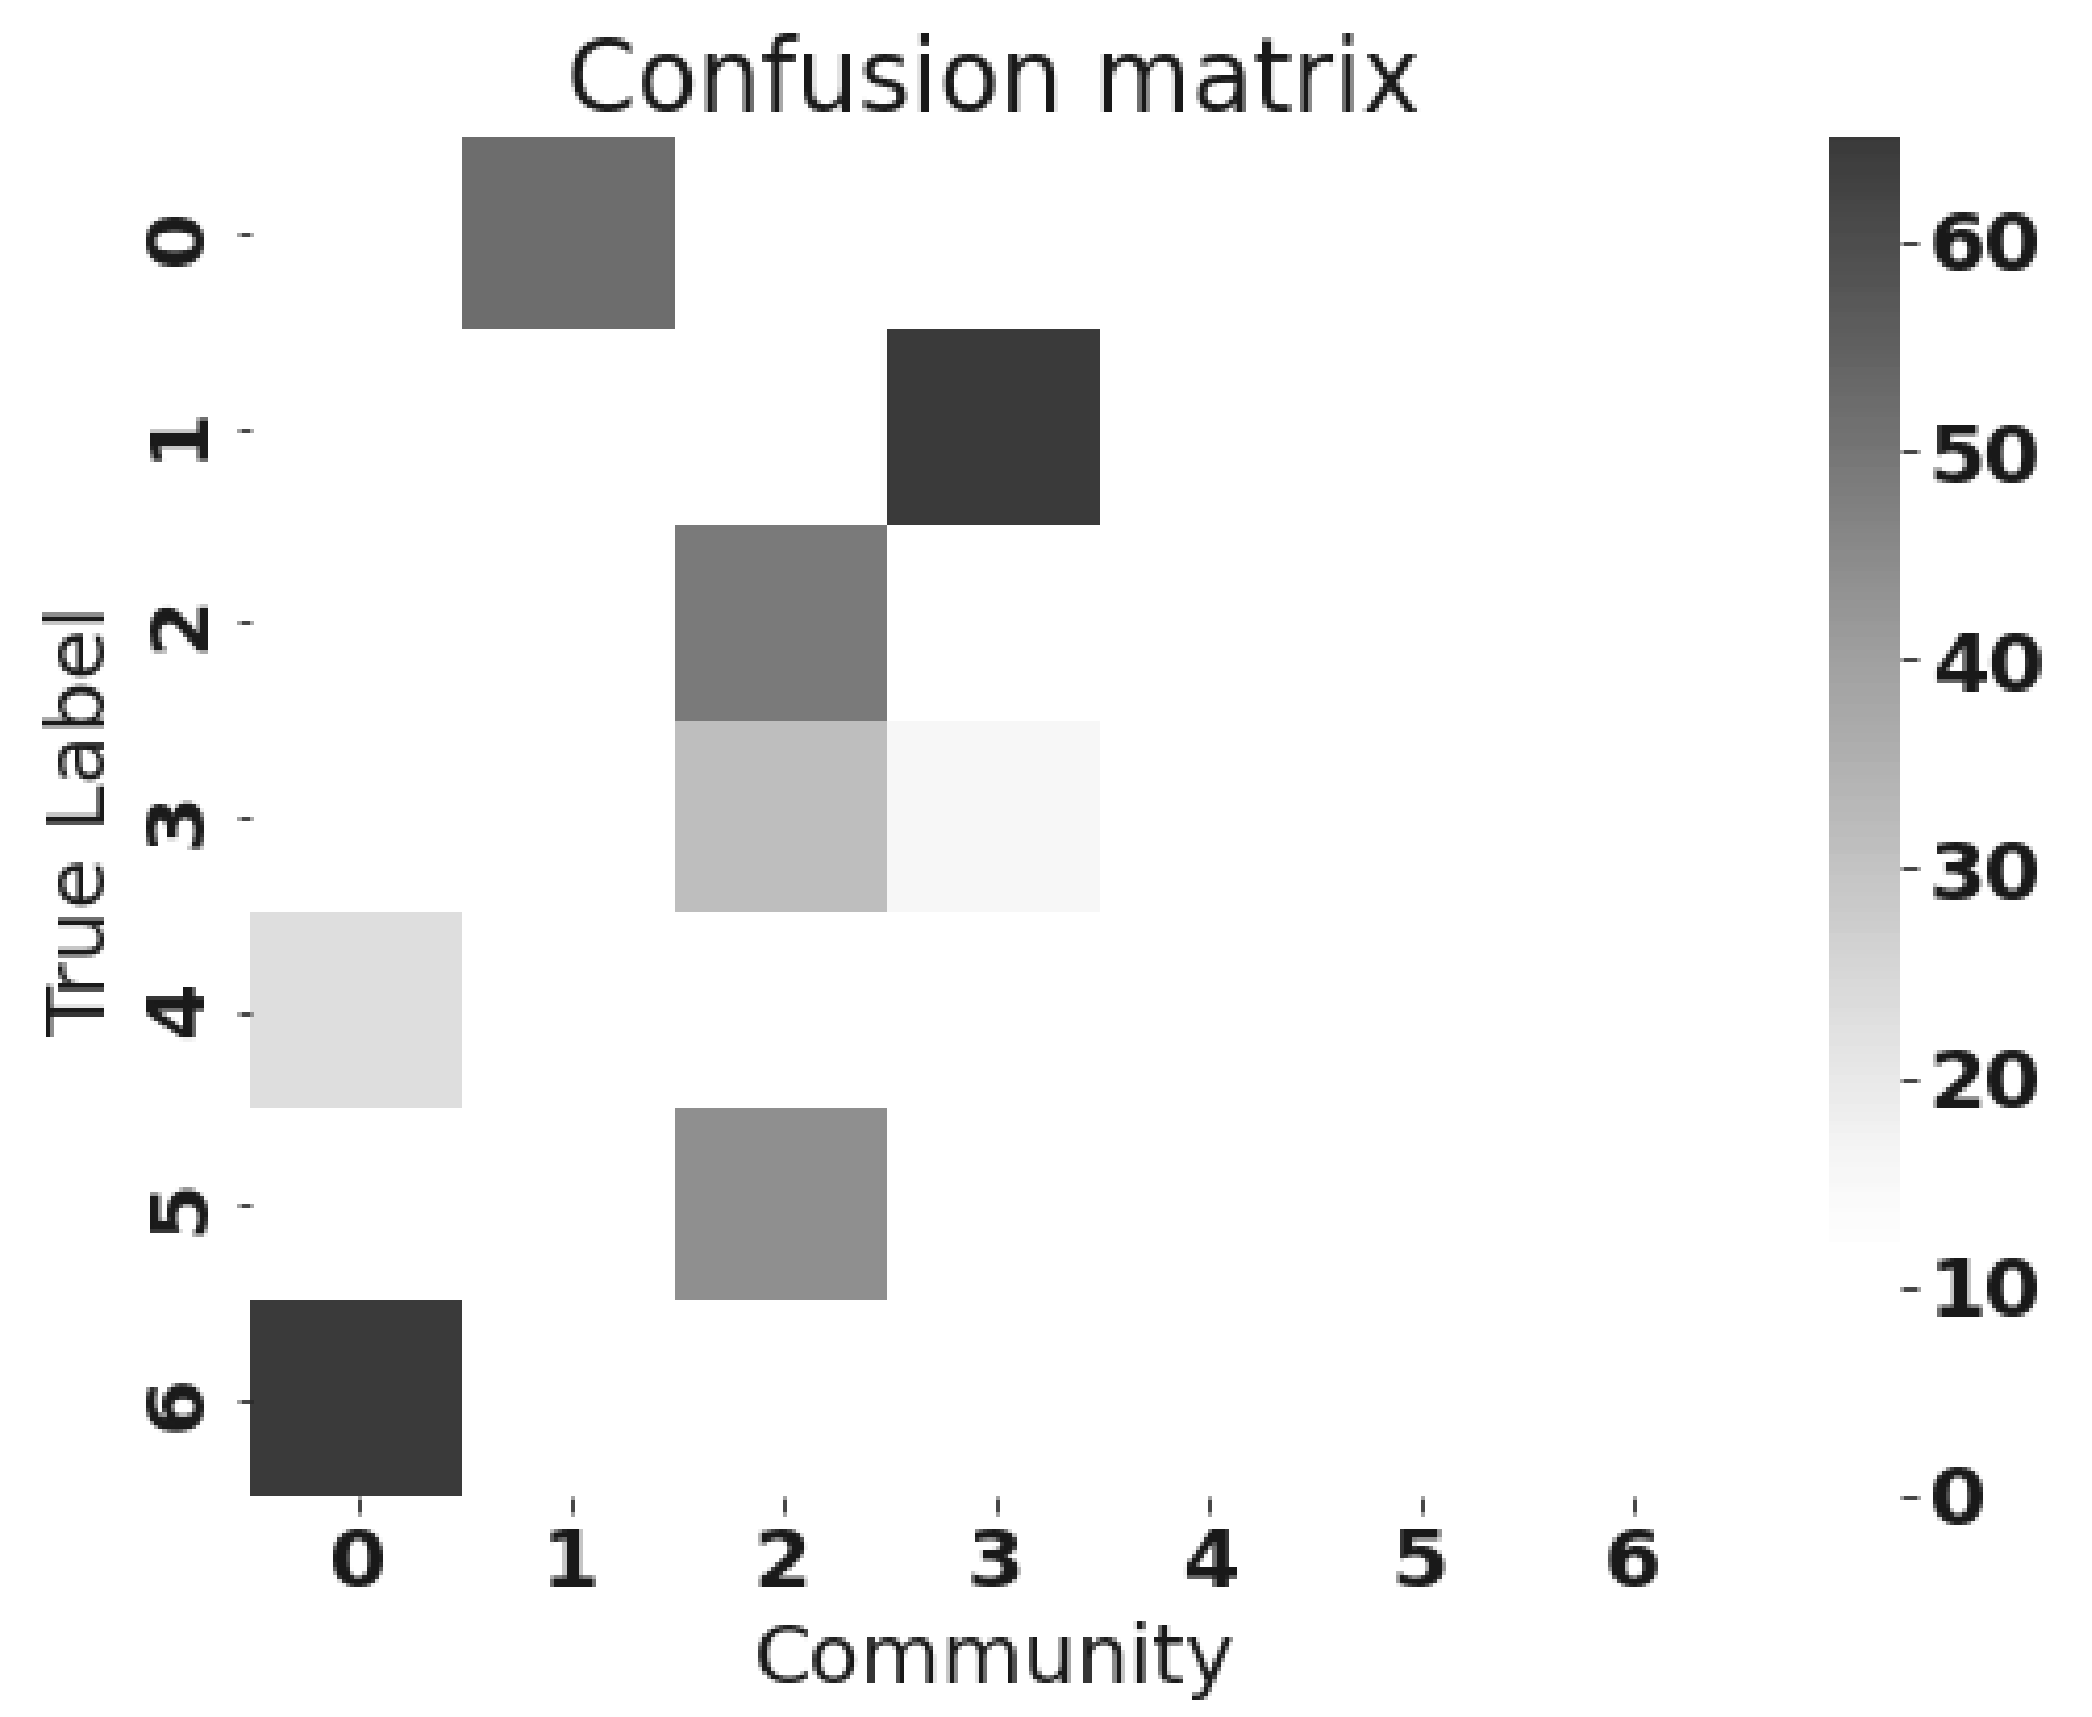
\includegraphics[width=0.5\linewidth]{foundations/ch2/Images/cf_mtx.png}
    \caption[Confusion matrix for node predictions]{The confusion matrix of the estimated clusters for each node in the networks, compared to the lobe that each node is in.}
    \label{fig:ch2:cf_mtx}
\end{figure}
The resulting plot is shown in Figure \ref{fig:ch2:cf_mtx}. in As you will learn in the section on \texttt{MASE} embedding in Section \ref{ch6:multinet:mase}, the mase embedding followed by clustering tends to find groups of nodes that have similar connectivity patterns in the connectomes (it will do a good job at finding the nodes that work together). This means that the nodes in the same community tend to behave ``as a unit'', if you will, in that they tend to be active/inactive together. Basically, what the plot above shows is that nodes that tend to have similar connectivity patterns (from the networks) tend to also be in the same parcel (the \emph{true label}), which makes sense since the parcels are based on connectivity profiles from brains. The clustering isn't \emph{perfect}, in that it is never the case that a single predicted label corresponds to \emph{exactly} one true label. If that were the case, we would expect for each column in the above ``confusion matrix'' to only have one possible true label that nodes within this predicted label are assigned to, which isn't quite the case. 

Taking these conclusions together, we find that some areas of the brain (such as the occipital and parietal areas) feature nodes which are both functionally \emph{and} spatially similar: they tend to show similar connectivity patterns with respect to other groups of nodes in the network, \emph{and} are in similar spatial positions in the brain. On the other hand, for other areas of the brain, while the nodes may be functionally similar, they might not necessarily be spatially similar. This is where the domain expertise kicks in: we don't know how to interpret this particular aspect of our finding, but maybe you or your colleagues do!

Further, while this analysis \emph{only} really ended up looking at whether different groups of nodes worked together, there's really no reason we couldn't \emph{also} incorporate spatial information about the nodes into our analysis. In Section \ref{sec:ch6:joint}, you will learn some techniques for incorporating both the network data itself and other information about the nodes into your analysis through a technique called Covariate-Assisted Spectral Embedding (\texttt{CASE}), such as spatial information.

And this is where the fun of network machine learning comes into play: it is a tool not only to \emph{apply} algorithms to data, but to facilitate \emph{learning new things} about that data as well. You might get some predictable conclusions (such as some of the nodes being both functionally and spatially similar), and you might get some unpredictable conclusions (such as some of the nodes being functionally, but \emph{not} spatially, similar). Your ability to understand network machine learning, while crucial, is going to go \emph{hand in hand} with your ability to understand the intricacies of the domain you want to apply network machine learning to. We hope that we can help with the former part; we'll leave the latter to you!

\subsection{Try it out}

Hopefully this chapter gave you a small scale peek at what a network machine learning project looks like, and showed you a brief introduction to some tools you can use to gain novel insights from your network data. While what we did in this chapter was relatively straightforward, the process from obtaining your data to choosing appropriate network machine learning problems can be extremely arduous! In fact, as a network machine learning scientist, you might find that just obtaining your data in a useful form (a network) and cleaning the data to be usable might take an \emph{enormous} chunk of your time!

If you haven't already done so, now is a fantastic time to grab your laptop, select a network dataset you are interested in, and start trying to work through the whole process from A to Z. If you need some pointers, the \texttt{graspologic} package makes several datasets available to you \cite{graspydata}. We'd recommend working through the contents of this book by first using the example data that is presented in the chapter, and then try to apply the techniques to a network dataset of your choosing.